\documentclass{wsdcr}
\usepackage[backend=bibtex]{biblatex}

\addbibresource{rapport.bib}

\title{Étude du model Lotka-Volterra}
\author{Robin Botrel, Axel Carpentier}
\affil{\textit{Université Paul Sabatier}\\
\textit{Toulouse, France}}
\date{28 Decembre, 2022}

\begin{document}

\maketitle
\tableofcontents
\section{Introduction}

\lettrine{C}{ette} étude des équations de prédation de Lotka-Volterra s'effectue dans le cadre d'une unité d'enseignement ouverte de la licence de mathématique de l'université Paul Sabatier. Nous allons partir d'un exercice vu en cours d'équations différentielles ordinaires (EDO), pour ensuite s'éloigner des frontières de ce cours et voir ce que peut offrir la discipline.


\subsection{Le model classique proie prédateur}

Les équations de Lotka-Volterra qualifient un système d'équations différentielles non linéaires, historiquement développées au début du 20ème siècle pour modéliser les interactions entre espèces et plus particulièrement entre 2 espèces : une proie et un prédateur, elles sont un exemple classique d'EDO. Le système est décrit équation \ref{eq:lotka-volterra}. \cite{lotka1920}
\begin{equation}
\left\{
{\begin{array}{ccc}{\dfrac {\mathrm {d} x(t)}{\mathrm {d} t}}&=&x(t)\ {\Big (}\alpha -\beta y(t){\Big )}\\{\dfrac {\mathrm {d} y(t)}{\mathrm {d} t}}&=&y(t)\ {\Big (}\delta x(t)-\gamma {\Big )}\end{array}}
\right.
\label{eq:lotka-volterra}
\end{equation}

%% the title 
\begin{center}
    \fontsize{10}{12}\fontfamily{phv}\fontshape{sc}\selectfont
    \textbf{Un peu d'histoire des mathématiques}
\end{center}

Dans sa publication de 1920 (c'est la première appartion sous cette forme de l'équation \ref{eq:lotka-volterra}), Lokta introduit son model comme un simple cas particulier d'interaction entre deux espèces : La source de nourriture de l'espèce 1 (notée $S_1$) est en excès et peut donc être considérée constante sur la période donnée. l'espèce $S_2$ se nourrit exclusivement de $S_1$.
Il introduit son raisonnement, $X_i$ est la masse de l'espèce $S_i$ :
\begin{equation}
\begin{aligned}
&\begin{bmatrix}
\text{Variation de }X_1 \\ \text{par unité de temps}
\end{bmatrix}
=
\begin{bmatrix}
X_1\text{ engendré}\\ \text{par unité de temps}
\end{bmatrix} \\
&- 
\begin{bmatrix}
X_1\text{ détruit par }X_2\\ \text{par unité de temps}
\end{bmatrix}
-
\begin{bmatrix}
\text{autre perte de }X_1\\ \text{par unité de temps}
\end{bmatrix} \\
&\begin{bmatrix}
\text{Variation de }X_2 \\ \text{par unité de temps}
\end{bmatrix}
=
\begin{bmatrix}
X_2\text{ engendré par l'ingestion de }X_1\\ \text{par unité de temps}
\end{bmatrix} \\
&-
\begin{bmatrix}
\text{autre perte de }X_2\\ \text{par unité de temps}
\end{bmatrix} 
\end{aligned}
\end{equation}
Pour translater ce raisonnement en un système d'EDO, il va faire de nouvelles assomptions, citons Lotka :
\begin{quotation}
Pour de petits changements, le taux de formation de nouvelle matière d'une espèce donnée d'organisme dans des conditions déterminées est proportionnel à la masse existante de cette espèce. En d'autres termes, la croissance de la matière vivante est un processus typiquement "autocatakinetic". […]. La proportionnalité ne s'applique pas aux grandes variations de X1, X2, ce qui est dûment pris en compte dans la mesure où $A_1'$, est une fonction de $X_1$, $X_2$. […]. De même, la masse de $S_1$ détruite par $S_2$ qui s'en nourrit sera, pour de petites variations, proportionnelle à $X_2$ et aussi à $X_1$. Ce terme a donc été défini sous la forme $B_1X_1X_2$. Ici encore, les écarts de proportionnalité sont pris en charge par les variations de $B_1$ avec $X_1$ et $X_2$, variables dont $B_1$ est une fonction.
\end{quotation}
\begin{equation}
\begin{aligned}
{\dfrac {\mathrm {d} X_1(t)}{\mathrm {d} t}}&=A_1^\prime X_1-B_1X_1X_2-A_1^{\prime \prime}X_1\\
{\dfrac {\mathrm {d} X_2(t)}{\mathrm {d} t}}&=A_2X_1X_2-B_2X_2
\end{aligned}
\end{equation}
Il construit sa translation vers un système d'EDO sur l'idée de proportionnalité mais tout en traitant cette proportionnalité comme des fonctions du temps. Durant toute la publication il n'envisage pas d'en faire des constantes. C'est Volterra qui en 1926 dans des lettres à Umberto D'Ancona, décrit la même équation mais tel que AB soit fixes, c'est l'équation que l'on a décrite eq.\ref{eq:lotka-volterra}. Volterra ne semble pas connaître les résultats précédents de Lotka. \cite{volterra1926}

Ce système d'EDO est non linéaire autonome, solution analytique, figure, C inf, forme résolue ??

\subsection{Généralisation}
Carrying capacity…
\begin{equation}
\left\{
{\begin{array}{ccc}{\dfrac {\mathrm {d} x(t)}{\mathrm {d} t}}&=&x(t)\ {\Big (}a -b y(t)-c x(t){\Big )}\\{\dfrac {\mathrm {d} y(t)}{\mathrm {d} t}}&=&y(t)\ {\Big (}d x(t)-e -f y(t) {\Big )}\end{array}}
\right.
\end{equation}
N dimension…
\begin{equation}
\dfrac {\mathrm {d}}{\mathrm {d} t}X(t)=X(t) {\Big (}R+AX(t){\Big )}
\end{equation}
\section{Le cas 2D}
Plusieurs visualisations du système : trajectoire (flow?), Champ vectoriel (def)…
Points d'équilibres et importance
\begin{equation}
R={\begin{bmatrix}1\\1\end{bmatrix}}\quad A =-{\begin{bmatrix}1&1\\1&1\end{bmatrix}}
\label{eq:RSnInv}
\end{equation}
\subsection{Une étude des bifurcations}
Le système définit par \ref{eq:RSnInv} possède un comportement étonnant découlant de la non inversibilité de $A$. L'étude des bifurcations a pour object d'étudier l'évolution d'un système dynamique (entres autres ses points d'équilibres) en fonction d'un ou plusieurs paramètres autour d'un changement majeur du système. Il est intéressant dans notre cas d'introduire un paramètre dans $A$ \ref{eq:RSs}, rendant $A(s)$ inversible $\forall s \in \mathds{R}\setminus \{1,-1\}, |A(s)|=1-s^2 \neq 0 $.
\begin{equation}
R={\begin{bmatrix}1\\1\end{bmatrix}}\quad A(s) =-{\begin{bmatrix}1&s\\s&1\end{bmatrix}}
\label{eq:RSs}
\end{equation}
Étudions les points d'équilibres et leurs stabilités de ce système paramétrique \ref{eq:RSs}. 
\begin{equation}
\begin{aligned}
X(R+AX)\overset{!}{=}0 &\land (x_1 = 0 \lor x_2 = 0) \Rightarrow (X=(0,0) \text{(O)} \lor \\ &X=(1,0) \text{(M)}\lor X=(0,1) \text{(N)})\\
X(R+AX)\overset{!}{=}0 &\land (x_1 ´\neq 0 \land x_2 \neq 0 \land s=1) \Rightarrow x_2=1-x_1 \\
X(R+AX)\overset{!}{=}0 &\land (x_1 ´\neq 0 \land x_2 \neq 0 \land s=-1) \Rightarrow X=\varnothing \\
X(R+AX)\overset{!}{=}0 &\land (x_1 ´\neq 0 \land x_2 \neq 0 \land s \neq \pm 1) \Rightarrow X=-A^{-1}R \\ &=\frac{1}{1-s^2}\begin{bmatrix}1&-s\\-s&1\end{bmatrix}\begin{bmatrix}1\\1\end{bmatrix}=\frac{1}{1+s}\begin{bmatrix}1\\1\end{bmatrix} \text{(S)}
\end{aligned}
\label{eq:RSs}
\end{equation}
\begin{equation}
\begin{aligned}
J(f)_X &= \begin{bmatrix}r_1-2x_1-sx_2&-sx_1\\-sx_2&r_2-2x_2-sx_1\end{bmatrix} \\
J(f)_{O} &= \begin{bmatrix}1&0\\0&1\end{bmatrix} \\particular
J(f)_{M} &= \begin{bmatrix}-1&-s\\0&1-s\end{bmatrix} \\
J(f)_{N} &= \begin{bmatrix}1-s&0\\-s&-1\end{bmatrix} \\
J(f)_{S,s\neq \{1,-1\}} &= \frac{1}{1+s}A(s)
\end{aligned}
\end{equation}
À l'aide des Jacobiennes, nous pouvont étudier la stabilité de ces points fixes et donc le comportement local des trajectoires. Soit F un des points fixes. $f$ étant $\mathcal{C}^\infty$ effectuons un développement de taylor à l'ordre 1 en F, sachant que $f(t,F)=0$.
\begin{equation}
f(t,F+H)=J(f)_XH + \mathcal{O}(\|H\|^2) 
\end{equation}
En négligeant les termes d'ordres strictement supérieurs à un, on obtient une nouvelle équation différentielle linéaire, valable localement en F.
\begin{equation}
{\dfrac {\mathrm {d} F+H}{\mathrm {d} t}}={\dfrac {\mathrm {d} H}{\mathrm {d} t}}=J(f)_FH
\end{equation}
Le point fixe O est expansif ($\forall i, \lambda_i > 0$), $J(f)_{M} \land J(f)_{N}$ diagonalisable $\forall s \neq 2$ (voir preuve), Soit $s=2$ … (figure) \\
Soit $S\neq2 \Rightarrow \exists P \in GL(\mathbb{R}),D \in \mathcal{M}(\mathbb{R}) \text{diagonal}, M = P^{-1}DP$ on a alors ${\dfrac {\mathrm {d} Y}{\mathrm {d} t}}=DY$ avec $Y(t)=PH(t)$ $\lambda_{1,2}$ les valeurs propres, déterminant et trace sont invariants par changement de base et peuvent nous informer sur le signe des valeurs propres en dimension 2.
\begin{itemize}
	\item $s>1 \Rightarrow Det(J(f)_{M})>0 \land Tr(J(f)_{M})<0 \Rightarrow \lambda_i<0$ {\color{red}point stable}
	\item $s=1 \Rightarrow \lambda_1=0 \land \lambda_2=-1$ 
	\item $1>s>0 \Rightarrow Det(J(f)_{M})<0 \land Tr(J(f)_{M})>0 \Rightarrow \lambda_1<0 \land \lambda_2>0$ {\color{red}point selle}
	\item $s=0 \Rightarrow \lambda_1=-1 \land \lambda_2=1$ {\color{red}point selle}
	\item $s<0 \Rightarrow Det(J(f)_{M})<0 \land Tr(J(f)_{M})>0 \Rightarrow \lambda_1<0 \land \lambda_2>0$ {\color{red}point selle}
\end{itemize}
Le cas du point fixe N est similaire au point M. Intéressons nous maintenant au point S. Vérifions que $\forall s \in \mathds{R}\setminus \{1,-1\}$ $J(f)_{S}$ diagonalisable.$Det(J(f)_{S}-XId_2)=\frac{1}{1+s}(\frac{1-s}{1+s}+X)(1+X)$ le polynôme est scindé à racine simple $\forall s \neq 0$ dans le cas où $s=0$ la jacobienne est diagonale. Finalement, $J(f)_{S}$ est diagonalisable $\forall s \in \mathds{R}\setminus \{1,-1\}$. On peut alors étudier le signe du déterminant et de la trace en fonction de $s$ : $Det(J(f)_{S})=\frac{1-s}{1+s}$ et $Tr(J(f)_{S})=\frac{-2}{1+s}$.
\begin{itemize}
	\item $s>1 \Rightarrow Det(J(f)_{S})<0 \land Tr(J(f)_{S})<0 \Rightarrow \lambda_1<0 \land \lambda_2>0$ {\color{red}point selle}
	\item $1>s>-1 \Rightarrow Det(J(f)_{S})>0 \land Tr(J(f)_{S})<0 \Rightarrow \lambda_i<0$ {\color{red}point stable}
	\item $s<-1 \Rightarrow Det(J(f)_{S})<0 \land Tr(J(f)_{S})>0 \Rightarrow \lambda_1<0 \land \lambda_2>0$ {\color{red}point selle}
\end{itemize}
\begin{figure}[t!]
    \centering
    \includegraphics[width=\linewidth]{fig/lv2_bif3Dx10.eps}
    \caption{test}
    \label{fig:example}
\end{figure}
\section{Chaos en 4D}
\subsection{introduction aux attracteurs}
dimension d'apparition
\begin{equation}
R={\begin{bmatrix}1\\0.72\\1.53\\1.27\end{bmatrix}}\quad A =-{\begin{bmatrix}1&1.09&1.52&0\\0&0.72&0.3168&0.9792\\3.5649&0&1.53&0.7191\\1.5367&0.6477&0.4445&1.27\end{bmatrix}}
\end{equation}
\begin{figure}
    \centering
    \subfigure[]{\includegraphics[width=0.3\linewidth]{fig/lv4_ps4.png}} 
    \subfigure[]{\includegraphics[width=0.3\linewidth]{fig/lv4_cl4.png}} 
    \subfigure[]{\includegraphics[width=0.3\linewidth]{fig/lv4_ae4.png}}
    \caption{(a) $S=0.8$ (b) $S=0.95$ (c) $S=1$}
    \label{fig:subbif}
\end{figure}
\begin{figure}
    \centering
    \includegraphics[width=\linewidth]{fig/lv4_ae4.png}
    \caption{attracteur étrange définit par XXX}
    \label{fig:ae4}
\end{figure}
\begin{figure}
    \centering
    \includegraphics[width=\linewidth]{fig/lv4_cl4.png}
    \caption{cycle limite définit par XXX}
    \label{fig:cl4}
\end{figure}
\subsection{bifurcations}
\begin{equation}
R={\begin{bmatrix}1\\0.72\\1.53\\1.27\end{bmatrix}}\quad A =-{\begin{bmatrix}1&1.09s&1.52s&0\\0&0.72&0.3168s&0.9792s\\3.5649s&0&1.53&0.7191s\\1.5367s&0.6477s&0.4445s&1.27\end{bmatrix}}
\end{equation}
\begin{figure}[t!]
    \centering
    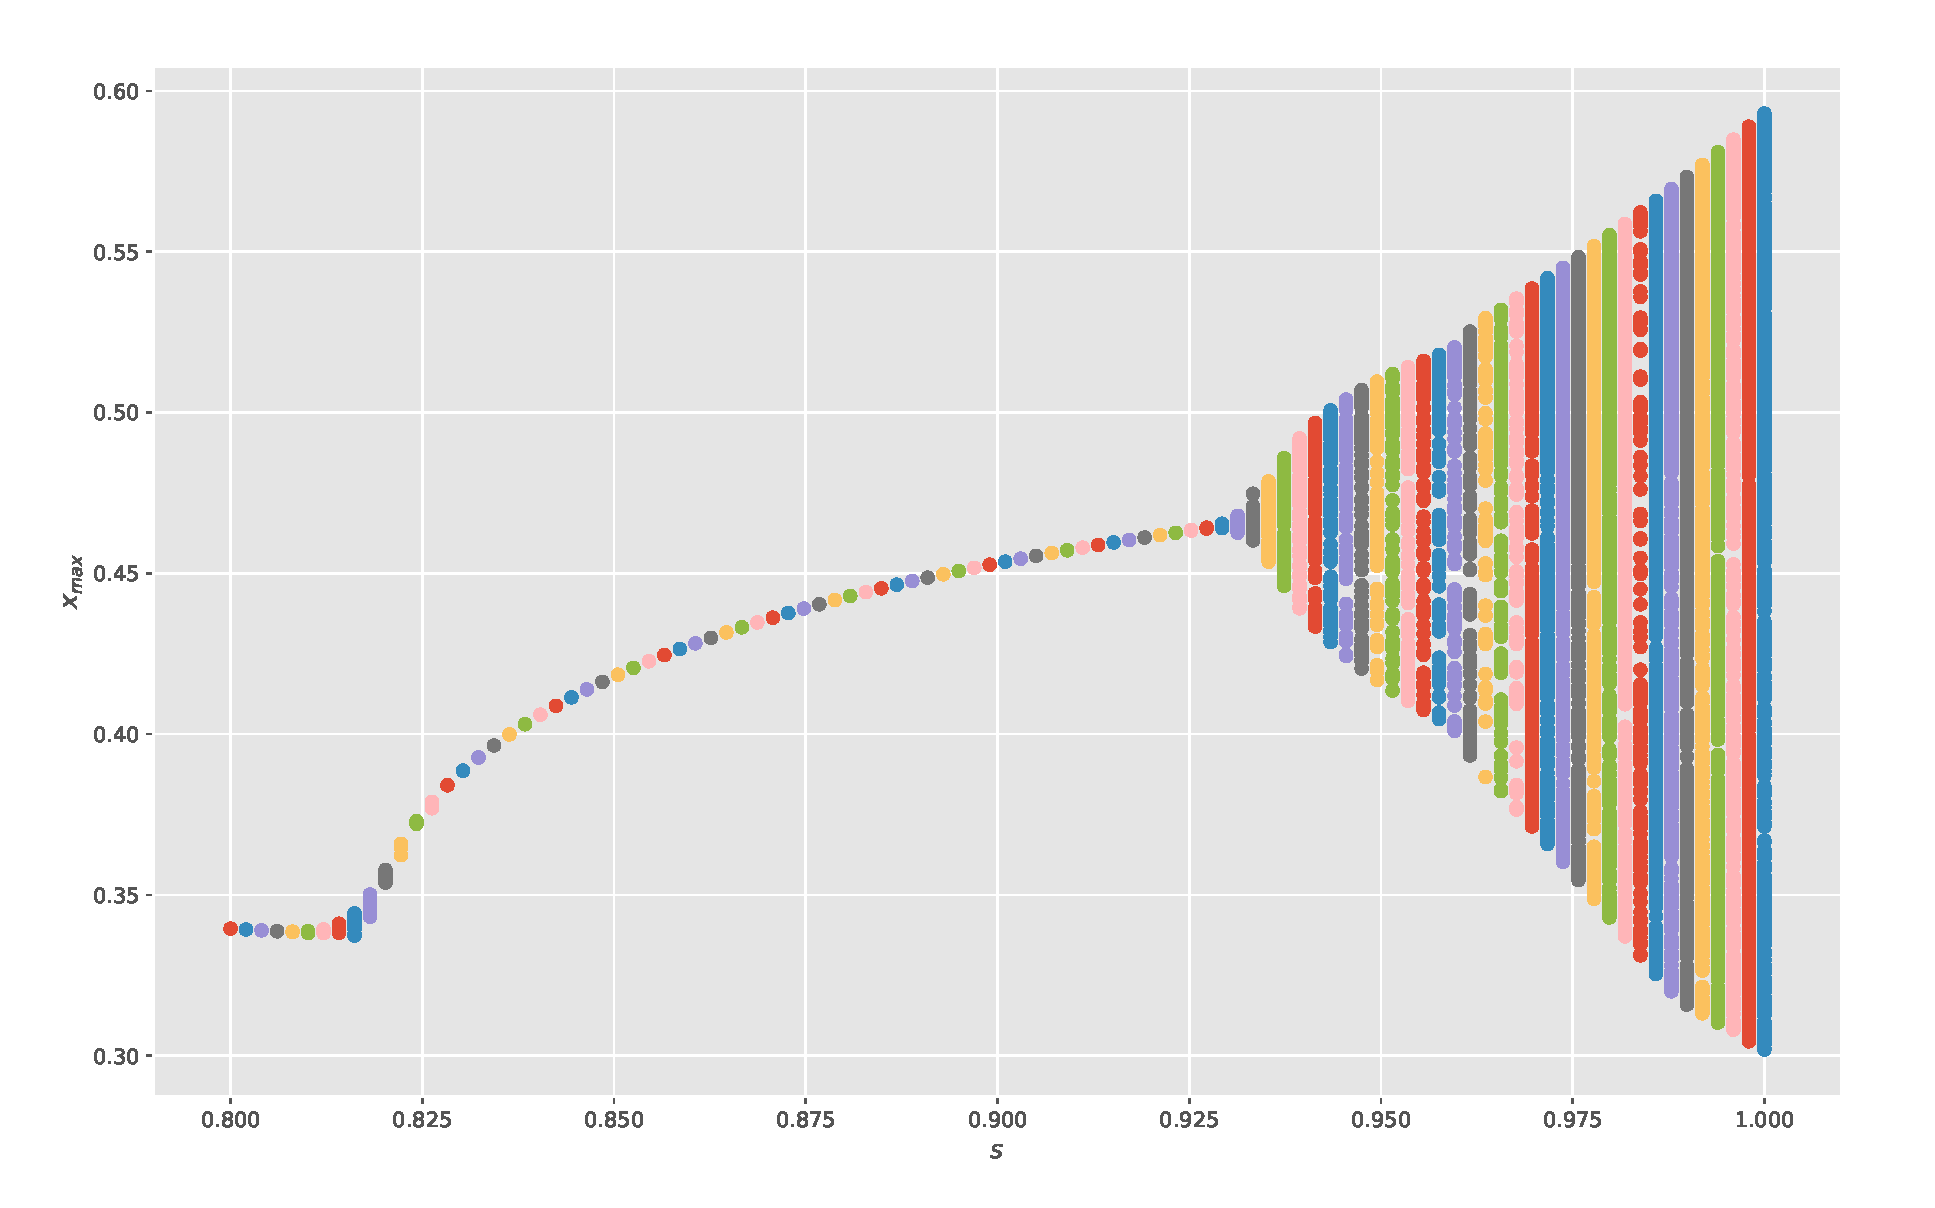
\includegraphics[width=\linewidth]{fig/lv4_bif.eps}
    \caption{test}
    \label{fig:bif4}
\end{figure}
\subsection{Cycle limite}
\begin{equation}
R={\begin{bmatrix}1\\0.72\\1.53\\1.27\end{bmatrix}}\quad A =-{\begin{bmatrix}1&1.0355&1.444&0\\0&0.72&0.30096&0.93024\\3.386655&0&1.53&0.683145\\1.459865&0.615315&0.422275&1.27\end{bmatrix}}
\end{equation}
\begin{figure}[t!]
    \centering
    \includegraphics[width=\linewidth]{fig/lv4_cl.png}
    \caption{test}
    \label{fig:example}
\end{figure}
\subsection{Exposant de Liapounov}
\section{Conclusion}

\section{Annexes}
\section{bibliographie}
\nocite{*}
\printbibliography



%
%\appendices


\end{document}
